\documentclass{UoNMCHA}
\usepackage[authoryear]{natbib}
\usepackage{array,booktabs} % For nice tables
\usepackage{amsmath,amsfonts,amssymb} % For nice maths
\usepackage{color}
\usepackage{enumerate}
\usepackage{listings}
\usepackage{subfig}
\usepackage{hyperref}
\usepackage[parfill]{parskip}   % For replacing paragraph indenting with a newline instead

% Number equations per section
\numberwithin{equation}{section}

\hypersetup{
%    bookmarks=true,         % show bookmarks bar?
%    unicode=false,          % non-Latin characters in AcrobatÕs bookmarks
%    pdftoolbar=true,        % show AcrobatÕs toolbar?
%    pdfmenubar=true,        % show AcrobatÕs menu?
%    pdffitwindow=false,     % window fit to page when opened
%    pdfstartview={FitH},    % fits the width of the page to the window
%    pdftitle={My title},    % title
%    pdfauthor={Author},     % author
%    pdfsubject={Subject},   % subject of the document
%    pdfcreator={Creator},   % creator of the document
%    pdfproducer={Producer}, % producer of the document
%    pdfkeywords={keyword1} {key2} {key3}, % list of keywords
%    pdfnewwindow=true,      % links in new window
    colorlinks=true,       % false: boxed links; true: colored links
    linkcolor=blue,          % color of internal links
    citecolor=blue,        % color of links to bibliography
%    filecolor=magenta,      % color of file links
    urlcolor=blue           % color of external links
}

\definecolor{MATLABKeyword}{rgb}{0,0,1}
\definecolor{MATLABComment}{rgb}{0.1328125,0.54296875,0.1328125}
\definecolor{MATLABString}{rgb}{0.625,0.125,0.9375}
\lstset{language=Matlab,
    basicstyle=\small\ttfamily,
    keywordstyle=\color{MATLABKeyword},
    %identifierstyle=,
    commentstyle=\color{MATLABComment},
    stringstyle=\color{MATLABString},
    numberstyle=\tiny,
    %numbers=left,
    basewidth=0.5em}
    
\definecolor{mGreen}{rgb}{0,0.6,0}
\definecolor{mGray}{rgb}{0.5,0.5,0.5}
\definecolor{mPurple}{rgb}{0.58,0,0.82}
\definecolor{backgroundColour}{rgb}{0.95,0.95,0.92}
\lstdefinestyle{CStyle}{
    backgroundcolor=\color{backgroundColour},   
    commentstyle=\color{mGreen},
    keywordstyle=\color{magenta},
    numberstyle=\tiny\color{mGray},
    stringstyle=\color{mPurple},
    % basicstyle=\footnotesize,
    basicstyle=\scriptsize\ttfamily,
    breakatwhitespace=false,         
    breaklines=true,                 
    captionpos=b,                    
    keepspaces=true,                 
    numbers=left,                    
    numbersep=5pt,                  
    showspaces=false,                
    showstringspaces=false,
    showtabs=false,                  
    tabsize=2,
    language=C
}

\firstpage{1}    % Set page number for first page
\UoNMCHAreportNo{AERO4600} %Report number
\UoNMCHAyear{2023}   % Year
\shorttitle{Report - AERO4600 Assignment X} %For odd pages
%%%%%%%%%%%%%%%%%%%%%%%%%%%%%%%%%%%%%%%%%%%%%%%%%%%%
\begin{document}
\title{AERO4600 Automatic Flight Control Systems\\
{\small Assignment 3 | 2024}}

\author[UoNMCHA]{Ben Miller}
\address[UoNMCHA]{
Student of Aerospace Systems Engineering,\\
The University of Newcastle, Callaghan, NSW 2308, AUSTRALIA \\
Student Number: c3328484 \\
E-mail: \href{mailto:First.Last@uon.edu.au}{\textsf{c3328484@uon.edu.au}}}

\author[UoNMCHA]{Jabez Mehanathan}
\address[UoNMCHA]{
Student of Aerospace Systems Engineering,\\
The University of Newcastle, Callaghan, NSW 2308, AUSTRALIA \\
Student Number: c3355997 \\
E-mail: \href{mailto:First.Last@uon.edu.au}{\textsf{c3355997@uon.edu.au}}}

\author[UoNMCHA]{Kaitlyn Ashcroft}
\address[UoNMCHA]{
Student of Aerospace Systems Engineering,\\
The University of Newcastle, Callaghan, NSW 2308, AUSTRALIA \\
Student Number: c3350754  \\
E-mail: \href{mailto:First.Last@uon.edu.au}{\textsf{c3350754@uon.edu.au}}}
%%%%%%%%%%%%%%%%%%%%%%%%%%%%%%%%%%%
\maketitle
\onecolumn

\vspace{-5mm}
\section*{Abstract}
\vspace{-3mm}
This Report examines the lateral dynamics and gust response of an aircraft and builds on prior work  \cite{A1-Report}, focusing on utilizing Matlab System Identification Toolbox as well as simulating aircraft response to gust inputs. The primary lateral modes analysed in this report are the side-slip ($\boldsymbol{\beta}$) and bank angle ($\boldsymbol{\phi}$) of the aircraft, and are evaluated through the influence of aileron/rudder control inputs and gust disturbances. This report also evaluates the impact of sensor noise on the the system identification model and methods of improving the robustness of the system identification process. Additionally, the gust/turbulence was modelled using the Dryden Spectra method to aid in simulating the gust responses, in order to compute the maximum side-slip and bank angle perturbations. These finding contribute to modelling and understanding the aircraft's dynamics and control in the lateral motion. 
\newpage
\tableofcontents
\newpage
%%%%%%%%%%%%%%%%%%%%%%%%%%%%%%%%%%%%%%%%%%%%%%%%%%%%%%%%%%%%%%
\section{Introduction}

\section{Q1 -- Vertical Speed Transfer Function}

\section{Q2 -- Pitch Rate Autopilot}

\section{Q3 -- Vertical Speed Guidance Loop}
The vertical speed guidance loop is designed to control the aircraft’s ascent and descent rates 
by incorporating a pitch rate controller as an inner loop. This loop includes a compensator in 
the forward leg, which processes the vertical speed error to generate a pitch rate command. 
The pitch rate command then feeds into the inner loop to modulate the elevator input, allowing 
the system to adjust vertical speed in response to deviations from the desired reference.

\subsection{Loop Topology}

\begin{figure}[ht!]
    \centering
    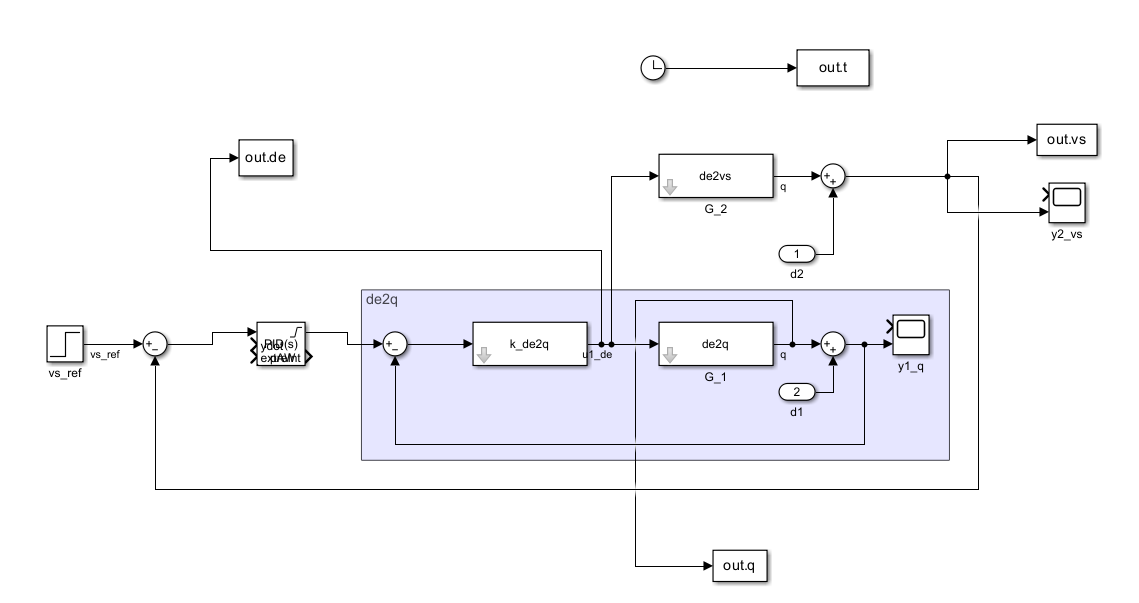
\includegraphics[width=1\linewidth]{Figures/Loop Topology -Q3.png}
    \caption{Caption}
    \label{fig:enter-label}
\end{figure}

\subsection{Aircraft Response to Vertical Speed Command}

\subsection{Pitch Rate Response}

\subsection{Elevator Activity}

\section{Q4 -- Design Auto-Throttle Control System}

\subsection{MIMO Loop Topology}

\subsection{Guidance Loop Topology Specifications}

\subsection{Primary Control Effects}

\subsection{Cross-coupling Control Effects}

\subsection{Elevator and Throttle Response}

\subsection{Auto-Throttle Effectiveness}

\section{Final Design}

\subsection{Q5 -- Implementation of the control and guidance laws}

\subsection{Q6 -- Gust Effectiveness}

\subsection{Q7 -- Commanded Large Vertical Speed}


\section{Conclusion}

%%%%%%%%%%%%%%%%%%%%%%%%%%%%%%%%
\bibliographystyle{harvard}
\bibliography{egBibtex} % This is the .bib file where the bibliography database is stored

\appendix
\newpage
\section{Example of a Table}\label{app:Table}
 %
\begin{table}[h!]
    \begin{center}\label{tab:MCHAProg}
        \caption{Bachelor of Engineering Mechatronics First Year Program}\label{tab:notation}
        {\footnotesize
            \begin{tabular}{c l l l|}
                \hline\hline \textbf{1st Year} & & \\
                Semester & {Course Code} & {Course Name} \\ \hline 
                1 & ENGG1003 & Introduction to Procedural Programming \\
                1 & ENGG1500 & Introduction to Professional Engineering\\
                1 & MATH1110 & Maths for Engineering, Science \& Technology 1 \\
                1 & MECH1110 & Mechanical Drawing/CAD \& Workshop Practice\\ \hline
                2 & CIVL1100 & Fundamentals of Engineering Mechanics\\
                2 & ELEC1310 & Introduction to Electrical Engineering\\
                2 & MATH1120 & Maths for Engineering, Science \& Technology 2 \\
                2 & MECH1750 & Engineering Materials I\\ \hline
            \end{tabular}
        }
    \end{center}
\end{table}

\end{document}
